\section{Results}

Primary analyses were divided into two phases: hypothesis testing and exploratory analyses. For the main hypothesis testing, paired sample t-tests were conducted on all outcome variables to assess overall changes from fall to spring within each academic year. Following this, exploratory analyses began by using mixed-design ANOVAs with the within-subject factor being time and the between-subject factor being participant characteristics (e.g., sex and returner status) to examine whether changes differed as a function of participant characteristics. This approach allowed for the detection of interaction effects that would not be captured by t-tests alone. When significant interactions were identified, simple effects analyses were conducted to probe the nature of the interaction, typically by comparing change over time within each subgroup or comparing groups at each time point using estimated marginal means. Since key participant characteristics were dichotomous, post-hoc comparisons were not required. Additional exploratory analyses used independent sample t-tests to compare differences between returners and new members’ baseline scores. 

Returners start with lower scores of anger inhibition in academic year 1 (AY1) compared to new members (see table~\ref{tab:T1Comparisons_AY1}).

%-----MAKE TABLE----%

\begin{table}[htbp]
\centering
\caption{Emotion Management and Resilience Measures by Membership Status at T1 in AY1}
\label{tab:T1Comparisons_AY1}
\begin{tabular}{lcccccccccc}
\hline
\textbf{Measure} & \multicolumn{3}{c}{\textbf{New Members}} & \multicolumn{3}{c}{\textbf{Returners}} & \textbf{$t$} & \textbf{df} & \textbf{$p$} & \textbf{Cohen's $d$} \\
\cline{2-4} \cline{5-7}
 & $N$ & $M$ & $SD$ & $N$ & $M$ & $SD$ & & & & \\ 
\hline
Anger Coping          & 26 & 12.35 & 1.94 & 14 & 11.64 & 1.86 & 1.11 & 38 & NS   & 0.37 \\
Anger Dysregulation   & 26 &  8.42 & 1.72 & 14 &  8.14 & 2.07 & 0.46 & 38 & NS   & 0.15 \\
Anger Inhibition      & 27 & 11.93 & 1.71 & 14 & 10.86 & 1.41 & 2.01 & 39 & .051 & 0.66 \\
Sad Coping            & 26 & 15.50 & 3.44 & 13 & 15.54 & 2.22 &-0.04 & 37 & NS   &-0.01 \\
Sad Dysregulation     & 24 &  8.88 & 1.65 & 13 &  9.31 & 0.85 &-0.88 & 35 & NS   &-0.30 \\
Sad Inhibition        & 25 & 11.80 & 1.85 & 13 & 12.15 & 1.72 &-0.57 & 36 & NS   &-0.19 \\
Rugged Resilience     & 26 & 26.19 & 7.62 & 13 & 34.77 & 8.50 & 0.53 & 37 & NS   & 0.18 \\
\hline
\end{tabular}
\end{table}
%----END OF TABLE---%

Returners ($T1$: $M = 36.11$, $SE = 2.48$; $T2$: $M = 39.67$, $SE = 2.02$) compared to new members ($T1$: $M = 37.47$, $SE = 1.92$; $T2$: $M = 34.53$, $SE = 1.57$) experienced greater gains in resilience scores, $F(1, 22) = 4.51$, $p = .054$, $\eta^2 = .159$ (see Figure~\ref{fig:Interaction_RRM}). Means from T1 and T2 of each group can also been seen in the bar graph (see Figure~\ref{fig:Bar_RRM}).

%----FIGURE PICTURE----%
\begin{figure}[H] 
\centering
\caption{\label{fig:Interaction_RRM} Time x Group Interaction for Rugged Resilience in Academic Year One}
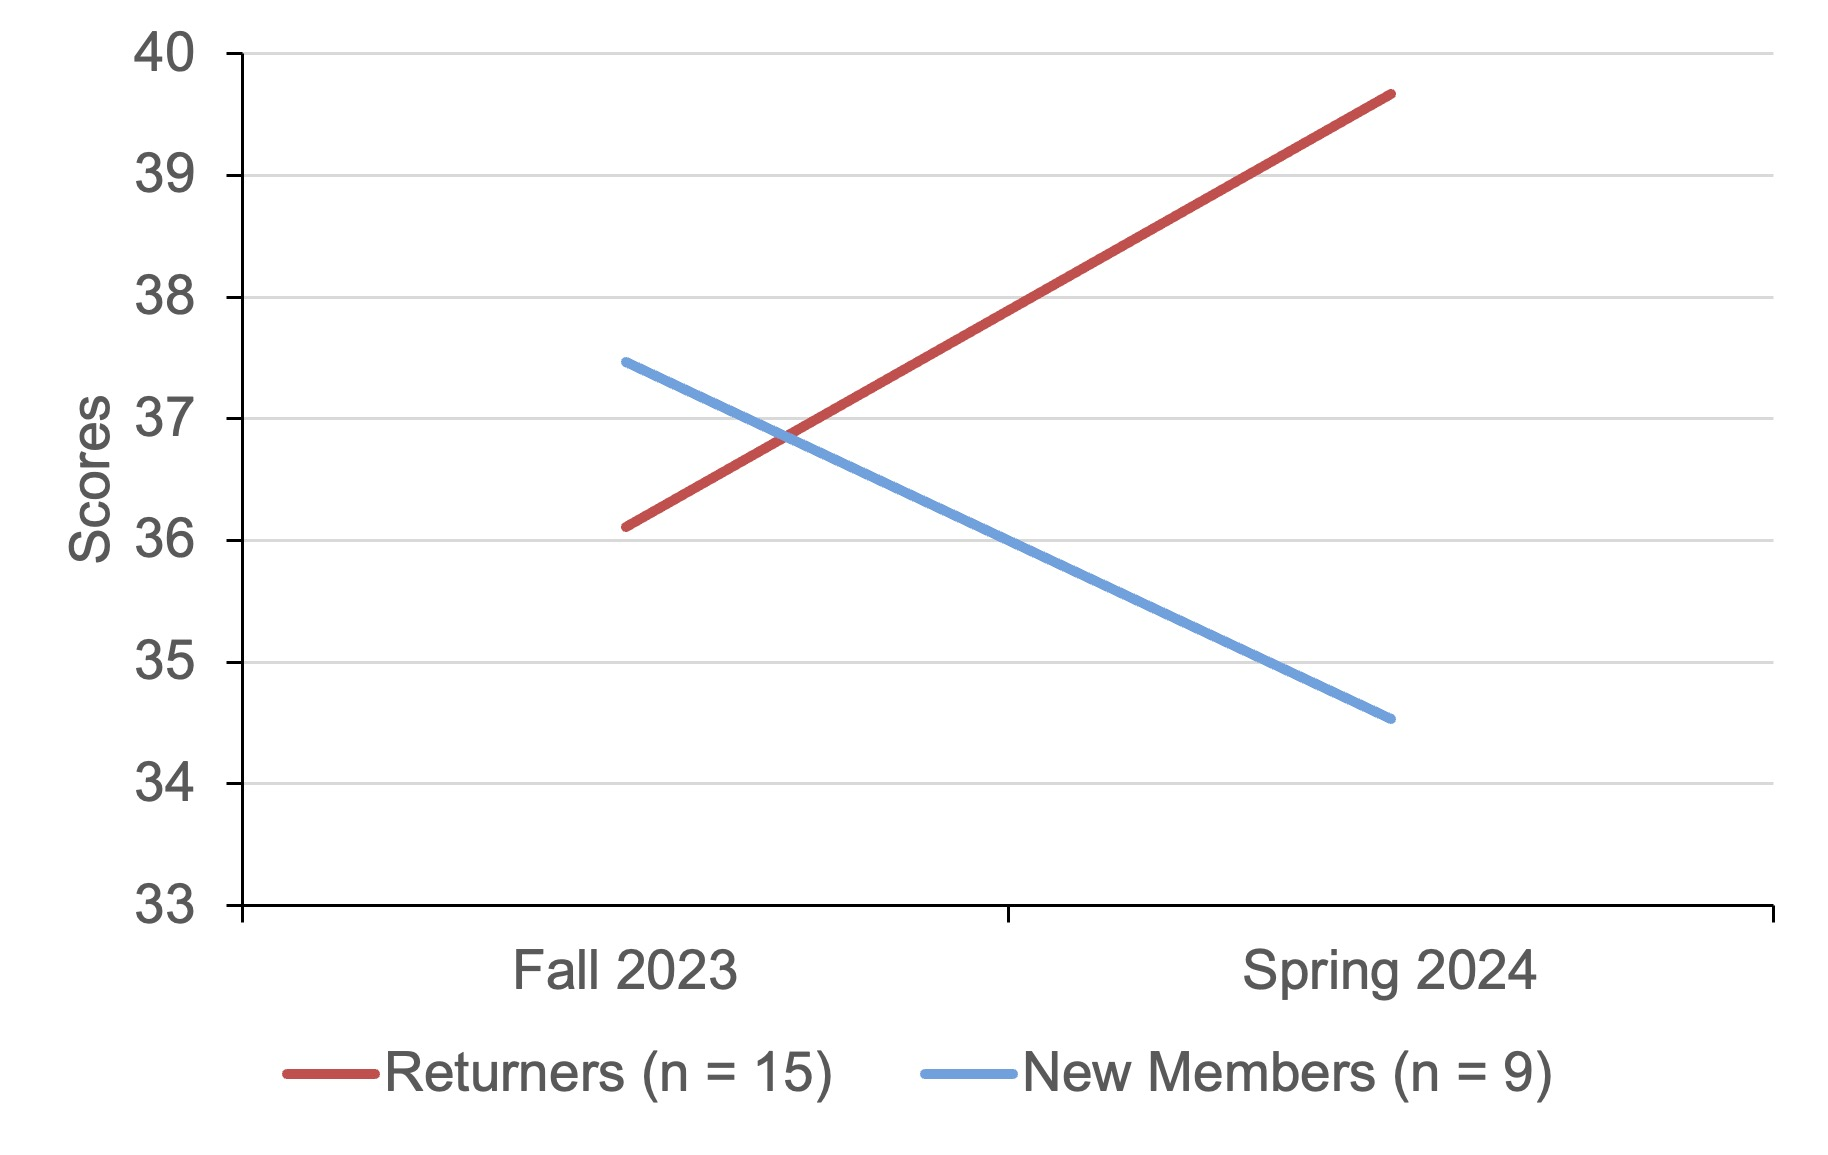
\includegraphics[width=0.8\textwidth]{LaTeXFigure1.jpg}
\captionsetup{font=small}
    \caption*{\textit{Note}. $F(1, 22) = 4.51$, $p = .054$, $\eta^2 = .159$.}
\end{figure}
%----END FIGURE PICTURE----%

%-----TikZ Picture----%
\begin{figure}[h!]
\centering
\caption{\label{fig:Bar_RRM} Mean Rugged Resilience Scores for New Members and Returners Across Time}
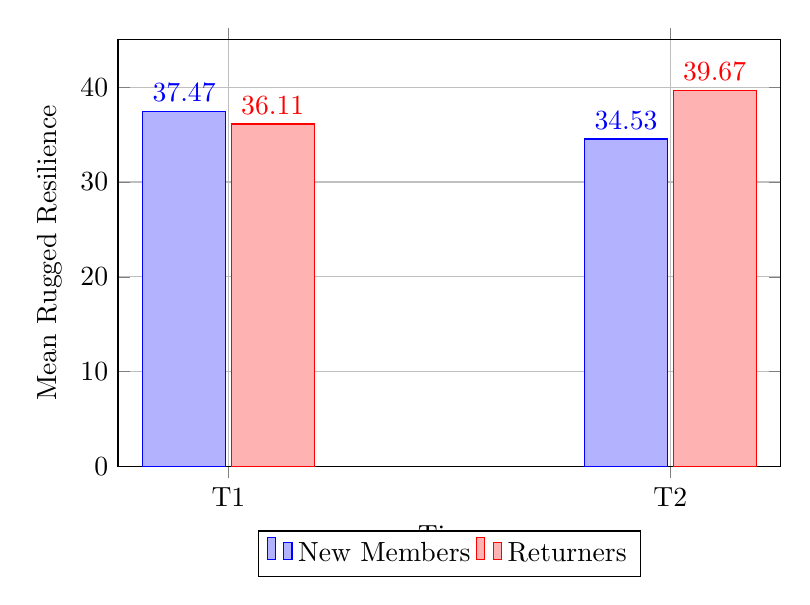
\begin{tikzpicture}
\begin{axis}[
    ybar,
    bar width=30pt,
    width=10cm,
    height=7cm,
    xlabel={Time},
    ylabel={Mean Rugged Resilience},
    symbolic x coords={T1,T2},
    xtick=data,
    ymin=0, ymax=45,
    legend style={at={(0.5,-0.15)}, anchor=north, legend columns=2},
    nodes near coords,
    nodes near coords align={vertical},
    grid=both,
    enlarge x limits=0.25,
]
\addplot coordinates {(T1,37.47) (T2,34.53)};
\addplot coordinates {(T1,36.11) (T2,39.67)};
\legend{New Members, Returners}
\end{axis}
\end{tikzpicture}
\captionsetup{font=small}
\caption*{\textit{Note}. $F(1, 22) = 4.51$, $p = .054$, $\eta^2 = .159$.}
\end{figure}
